\graphicspath{{figs/3b}}

\chapter{Approximate Inference in Classification}
\section{Bayesian Logistic Regression}
\subsection{Maximum-A-Posteriori Estimate}
\paragraph{1.1. Analyze the results provided by previous plot. Looking at $p(\mathbf{y}=1 | \pmb{x}, \pmb{w}_{\textrm{MAP}})$, what can you say about points far from train distribution?}
In Figure \ref{fig:bayes_MAP}, which illustrates Bayesian Logistic Regression applied to a binary classification dataset, we can see two clusters of data points, one represented in blue and the other in red, corresponding to different classes. The shaded regions, in blue and red, depict the predictive uncertainty associated with each class. The lighter shade indicates lower confidence in the model's predictions.

Approximating $p(\mathbf{w} | \mathbf{X}, \mathbf{Y})$ with a Dirac delta function is essentially akin to approximating the predictive distribution using $\mathbf{w}_{\textrm{MAP}}$, meaning $p(y=1 | \mathbf{x}, \mathbf{w}_{\textrm{MAP}}) \approx p(y=1 | \mathbf{x}, \mathbf{Y})$. This approximation is quite rudimentary.

As depicted in Figure \ref{fig:bayes_MAP}, the model's uncertainty doesn't significantly increase far from the training data. This limitation indicates that the point-wise estimate of the parameters can only confidently assign points to their respective classes but lacks the capacity to provide nuanced uncertainty measures for points that deviate far from the training data distribution.

\begin{figure}[H]
    \centering
    % 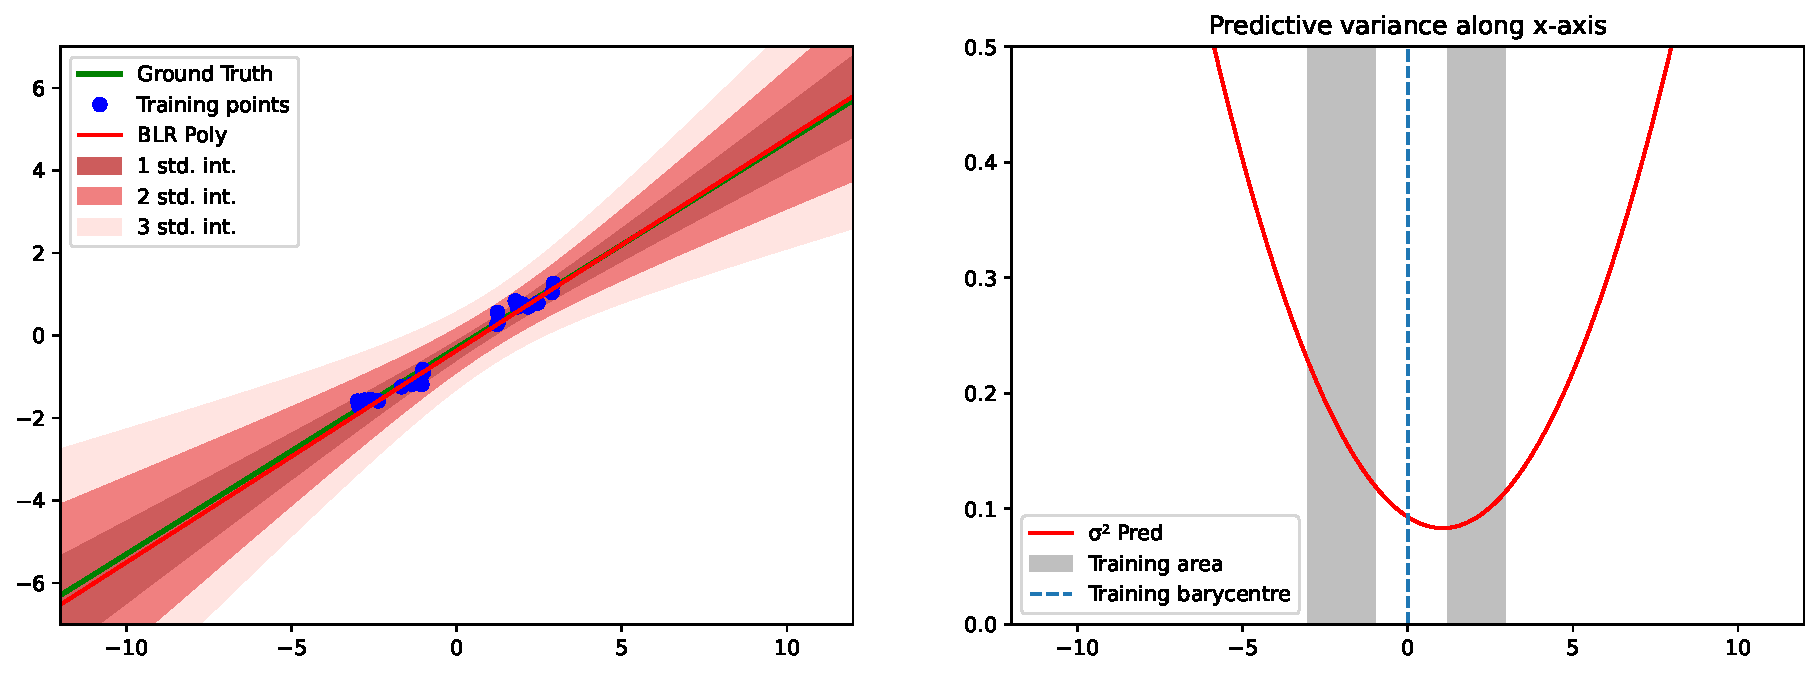
\includegraphics[width=0.95\textwidth]{phi_linear_hole.pdf}
    \caption{Illustration of a Bayesian Logistic Regression model applied to a binary classification task with uncertainty display. Two distinct data point clusters — blue and red — represent separate classes, while the surrounding shaded areas reflect the model's predictive uncertainty, with lighter shades indicating lower confidence. The model exhibits a limitation in uncertainty estimation, remaining overconfident far from the training data, hence lacking in providing nuanced uncertainty measures for outlying points.}
    \label{fig:bayes_MAP}
\end{figure}

\subsection{Laplace Approximation}
\paragraph{1.2. Analyze the results provided by previous plot. Compared to previous MAP estimate, how does the predictive distribution behave?}

\paragraph{1.3. Comment the effect of the regularisation hyper-parameter  \texttt{WEIGHT\_DECAY}.}

\subsection{Variational Inference}
\paragraph{1.4. Comment the code of the \texttt{VariationalLogisticRegression} and \texttt{LinearVariational} classes.}
= answer to see if we understand what the code does

\paragraph{1.5. Comment the code of the training loop, especially the loss computation. Analyze the results provided by previous plot. Compared to previous MAP estimate, how does the predictive distribution behave? What is the main difference between the Variational approximation and the Laplace approximation?}

\section{Bayesian Neural Networks}
\subsection{Variational Inference with Bayesian Neural Networks}
\paragraph{2.1. Analyze the results showed on plot.}

\subsection{Monte Carlo Dropout}
\paragraph{2.2. Again, analyze the results showed on plot. What is the benefit of MC Dropout variational inference over Bayesian Logistic Regression with variational inference?}